\section{Loads on the structure}
\label{sec:loads}

\begin{keybox}
\begin{itemize}
\item The pressure pushes the shell \textbf{inward only at the front}: on the rounded tip at burnout (up to
\val{B-hot-LC1-dpstag}\,kPa), and on design A over the first few centimetres (up to
\val{A-hot-LC1-dpmax2}\,kPa). From mid-length to the shoulder the net pressure is \textbf{never inward}.
\item The \textbf{outward} pressure grows during the whole climb as the outside air gets thinner. At
apogee it is about \absval{A-nominal-LC3-dpmin}\,kPa on the whole shell, for both designs.
\item \textbf{Along the axis, the sealed nose is pulled off the joint at every load case.} The
overpressure inside outweighs the drag already at burnout, and at apogee the pull reaches about
\absval{B-hot-LC3-Fphi}\,N.
\item \textbf{Side force}: \val{A-nominal-LC1-Nperdeg}\,N per degree of angle of attack at burnout
(\val{B-hot-LC1-Nperdeg}\,N on a hot day), the same for both designs. It acts \val{A-xcp}\,mm (A) or
\val{B-xcp}\,mm (B) behind the tip.
\end{itemize}
\end{keybox}

\subsection{Pressure along the nose, at the three load cases}
\label{sec:pressure}

At the tip the oncoming air is stopped and presses hard on the rounded cap. The pressure falls quickly
over the first few millimetres. Further back the wall pressure is close to the outside pressure, and
slightly below it towards the shoulder, where the air speeds up onto the cylinder. The inside stays at
the pad pressure, so the rear half of the shell is pushed outward at every load case
(Figure~\ref{fig:dpx}). Over the first 10\,cm design A, with its fuller front, has about twice the
pressure of design B.

\begin{figure}[H]
\centering
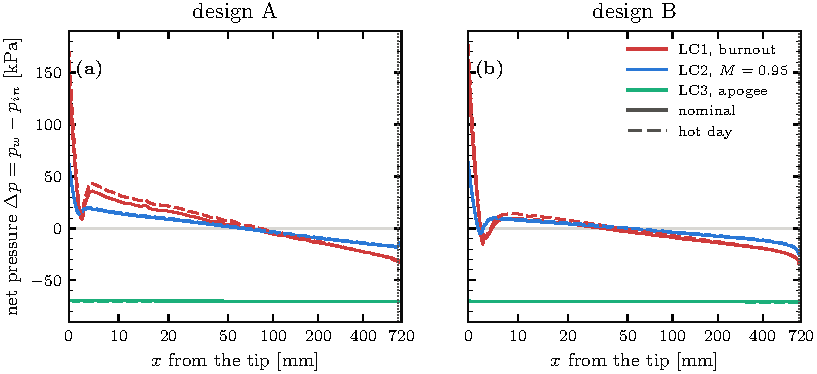
\includegraphics[width=\linewidth]{fig_dp_x}
\caption{Net pressure along the nose at the three load cases, design A (a) and design B (b). Above zero
the shell is pushed inward, below zero outward. Solid: nominal day; dashed: hot day. The $x$ axis is
stretched near the tip (logarithmic beyond 20\,mm); the dotted line is the shoulder.}
\label{fig:dpx}
\end{figure}

\begin{table}[H]
\centering
\caption{Net pressure at the three load cases [kPa]. Positive: inward, with cold inside air. Negative:
outward, with heated inside air. Each bound is the one that gives the larger load.}
\label{tab:dp_lc}
\small
\begin{tabular}{@{}lccccc@{}}
\toprule
 & \multicolumn{2}{c}{Design A} & \multicolumn{2}{c}{Design B}\\
\cmidrule(lr){2-3}\cmidrule(l){4-5}
 & Nominal & Hot day & Nominal & Hot day\\
\midrule
\grouprow{5}{LC1, burnout}
On the rounded tip (inward) & \val{A-nominal-LC1-dpstag} & \val{A-hot-LC1-dpstag} & \val{B-nominal-LC1-dpstag} & \val{B-hot-LC1-dpstag}\\
Highest behind the tip, $x > 2$\,mm (inward) & \val{A-nominal-LC1-dpmax2} & \val{A-hot-LC1-dpmax2} & \val{B-nominal-LC1-dpmax2} & \val{B-hot-LC1-dpmax2}\\
Lowest on the shell (outward) & \val{A-nominal-LC1-dpmin} & \val{A-hot-LC1-dpmin} & \val{B-nominal-LC1-dpmin} & \val{B-hot-LC1-dpmin}\\
\midrule
\grouprow{5}{LC2, transonic}
On the rounded tip (inward) & \val{A-nominal-LC2-dpstag} & \val{A-hot-LC2-dpstag} & \val{B-nominal-LC2-dpstag} & \val{B-hot-LC2-dpstag}\\
Highest behind the tip, $x > 2$\,mm (inward) & \val{A-nominal-LC2-dpmax2} & \val{A-hot-LC2-dpmax2} & \val{B-nominal-LC2-dpmax2} & \val{B-hot-LC2-dpmax2}\\
Lowest on the shell (outward) & \val{A-nominal-LC2-dpmin} & \val{A-hot-LC2-dpmin} & \val{B-nominal-LC2-dpmin} & \val{B-hot-LC2-dpmin}\\
\midrule
\grouprow{5}{LC3, apogee}
Whole shell (outward) & \val{A-nominal-LC3-dpmin} & \val{A-hot-LC3-dpmin} & \val{B-nominal-LC3-dpmin} & \val{B-hot-LC3-dpmin}\\
\bottomrule
\end{tabular}
\end{table}

\subsection{Pressure during the flight, at four stations}

Figure~\ref{fig:dpt} follows the net pressure at the four stations of Figure~\ref{fig:conventions}
through the whole flight, and Table~\ref{tab:stations} gives the extremes.
\begin{itemize}
\item The tip is pushed inward from lift-off until 15--17\,s, with the peak at burnout.
\item The other stations are pushed outward for almost the whole flight, more and more as the rocket
climbs.
\item When the shell heats the inside air, the inside pressure rises and adds a few kPa of outward
pressure during the coast (thin lines). At the shoulder of design B this gives the largest outward value
of the flight, \val{B-hot-stshoulder-min}\,kPa at \val{B-hot-stshoulder-tmin}\,s on the hot day.
\end{itemize}

\begin{figure}[H]
\centering
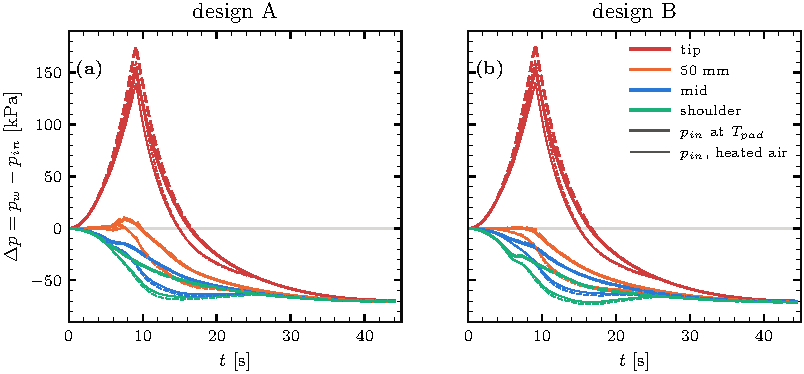
\includegraphics[width=\linewidth]{fig_dp_t}
\caption{Net pressure during the flight at the four stations, design A (a) and design B (b). Above zero
the shell is pushed inward. Thick: cold inside air; thin: heated inside air. Solid: nominal day; dashed:
hot day.}
\label{fig:dpt}
\end{figure}

\begin{table}[H]
\centering
\caption{Largest net pressure over the flight at the four stations [kPa]. Inward peaks: at the tip at
burnout, at 50\,mm at 7.2--7.5\,s ($M \approx 1.2$); 0 means never inward. Outward peaks: at apogee,
except the shoulder of design B (\val{B-hot-stshoulder-tmin}--\val{B-nominal-stshoulder-tmin}\,s).}
\label{tab:stations}
\small
\begin{tabular}{@{}lcccc@{}}
\toprule
 & \multicolumn{2}{c}{Design A} & \multicolumn{2}{c}{Design B}\\
\cmidrule(lr){2-3}\cmidrule(l){4-5}
 & Nominal & Hot day & Nominal & Hot day\\
\midrule
\grouprow{5}{Inward (cold inside air)}
Tip & \val{A-nominal-sttip-max} & \val{A-hot-sttip-max} & \val{B-nominal-sttip-max} & \val{B-hot-sttip-max}\\
50\,mm & \val{A-nominal-st50-max} & \val{A-hot-st50-max} & \val{B-nominal-st50-max} & \val{B-hot-st50-max}\\
Mid-length & \val{A-nominal-stmid-max} & \val{A-hot-stmid-max} & \val{B-nominal-stmid-max} & \val{B-hot-stmid-max}\\
Shoulder & \val{A-nominal-stshoulder-max} & \val{A-hot-stshoulder-max} & \val{B-nominal-stshoulder-max} & \val{B-hot-stshoulder-max}\\
\midrule
\grouprow{5}{Outward (heated inside air)}
Tip & \val{A-nominal-sttip-min} & \val{A-hot-sttip-min} & \val{B-nominal-sttip-min} & \val{B-hot-sttip-min}\\
50\,mm & \val{A-nominal-st50-min} & \val{A-hot-st50-min} & \val{B-nominal-st50-min} & \val{B-hot-st50-min}\\
Mid-length & \val{A-nominal-stmid-min} & \val{A-hot-stmid-min} & \val{B-nominal-stmid-min} & \val{B-hot-stmid-min}\\
Shoulder & \val{A-nominal-stshoulder-min} & \val{A-hot-stshoulder-min} & \val{B-nominal-stshoulder-min} & \val{B-hot-stshoulder-min}\\
\bottomrule
\end{tabular}
\end{table}

\subsection{Axial force on the joint}
\label{sec:forces}

Table~\ref{tab:axial} gives the \textbf{net pressure force} of the sealed nose: the outside wall pressure
minus the inside pressure, summed over the shell. It contains the pressure part of the drag and the pull
of the inside overpressure; friction is not in it. The \textbf{drag} of the nose, which is what a vented
nose would put on the joint, is in Section~\ref{sec:drag}.

\begin{table}[H]
\centering
\caption{Net pressure force on the joint at the three load cases [N]. Positive: compression, the nose is
pushed onto the joint. Negative: tension, the nose is pulled off the joint.}
\label{tab:axial}
\small
\begin{tabular}{@{}lcccc@{}}
\toprule
 & \multicolumn{2}{c}{Design A} & \multicolumn{2}{c}{Design B}\\
\cmidrule(lr){2-3}\cmidrule(l){4-5}
 & Nominal & Hot day & Nominal & Hot day\\
\midrule
\grouprow{5}{LC1, burnout}
Net pressure force, cold inside air & \val{A-nominal-LC1-Fplo} & \val{A-hot-LC1-Fplo} & \val{B-nominal-LC1-Fplo} & \val{B-hot-LC1-Fplo}\\
Net pressure force, heated inside air & \val{A-nominal-LC1-Fphi} & \val{A-hot-LC1-Fphi} & \val{B-nominal-LC1-Fphi} & \val{B-hot-LC1-Fphi}\\
\midrule
\grouprow{5}{LC2, transonic}
Net pressure force, cold inside air & \val{A-nominal-LC2-Fplo} & \val{A-hot-LC2-Fplo} & \val{B-nominal-LC2-Fplo} & \val{B-hot-LC2-Fplo}\\
Net pressure force, heated inside air & \val{A-nominal-LC2-Fphi} & \val{A-hot-LC2-Fphi} & \val{B-nominal-LC2-Fphi} & \val{B-hot-LC2-Fphi}\\
\midrule
\grouprow{5}{LC3, apogee}
Net pressure force & \val{A-nominal-LC3-Fphi} & \val{A-hot-LC3-Fphi} & \val{B-nominal-LC3-Fphi} & \val{B-hot-LC3-Fphi}\\
\bottomrule
\end{tabular}
\end{table}

At apogee the pull of about 1.8\,kN is close to the 2000\,N of Req\_07. Vent holes would bring the inside
pressure to the outside pressure and remove it; the air load on the joint would then be the drag only. The
inertial loads at the joint and the recovery load are not in this report.

\subsection{Side force under an angle of attack}
\label{sec:normal}

Fluent was run at zero angle of attack only. For a small angle of attack $\alpha$, slender-body theory gives
the side (normal) force of the nose and where it acts:
\begin{equation}
N = 2\,q\,A_{ref}\,\alpha \quad (\alpha \text{ in rad}), \qquad
M_b = N\,(x_j - x_{CP}),
\end{equation}
with $M_b$ the bending moment at the joint plane $x_j$. The force is carried mostly by the front half of the
nose (Figure~\ref{fig:normal}); the coupler carries none. ST chooses the design angle of attack (Req\_12).

\begin{table}[H]
\centering
\caption{Side force per degree of angle of attack, and its point of action.}
\label{tab:normal}
\small
\begin{tabular}{@{}llcccc@{}}
\toprule
\caseheader
\midrule
Side force at LC1, burnout & N/$^\circ$ & \val{A-nominal-LC1-Nperdeg} & \val{A-hot-LC1-Nperdeg} & \val{B-nominal-LC1-Nperdeg} & \val{B-hot-LC1-Nperdeg}\\
Side force at LC2, transonic & N/$^\circ$ & \val{A-nominal-LC2-Nperdeg} & \val{A-hot-LC2-Nperdeg} & \val{B-nominal-LC2-Nperdeg} & \val{B-hot-LC2-Nperdeg}\\
Centre of pressure $x_{CP}$, from the tip & mm & \multicolumn{2}{c}{\val{A-xcp}} & \multicolumn{2}{c}{\val{B-xcp}}\\
\bottomrule
\end{tabular}
\end{table}

\begin{figure}[H]
\centering
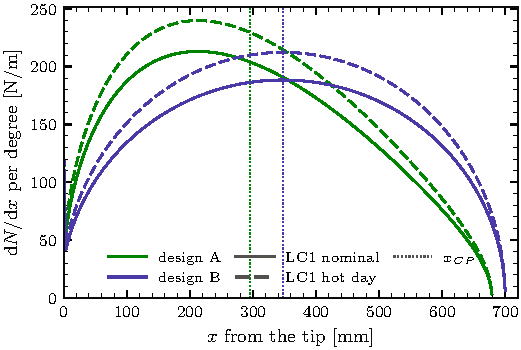
\includegraphics[width=0.75\linewidth]{fig_normal_load}
\caption{Side force per unit length and per degree of angle of attack at burnout (slender-body theory).
Dotted: centre of pressure.}
\label{fig:normal}
\end{figure}
